\documentclass[12pt]{article}

\usepackage{geometry}
\geometry{margin = .5in,top =0.12\paperheight, headheight=\paperheight}
\usepackage{array}
\usepackage{amsmath}
\usepackage{amsfonts}
\usepackage{amsthm}
\usepackage[export]{adjustbox}
\usepackage{fancyhdr}
\usepackage{lastpage}
\pagestyle{fancy}
\fancyhf{}
\rhead{Written Assignment, Page \thepage}
\lhead{MATH308}
\chead{
\includegraphics[width = 0.15\textwidth]{MCLogo-Bck.png}}
\usepackage{mathrsfs}

%\renewcommand{\footrulewidth}{0.4pt}

\usepackage{enumitem}
\usepackage{pifont}
\usepackage{graphicx}
\graphicspath{{../img}}

\newtheorem*{theorem}{Theorem}
\newtheorem{exercise}{Exercise}


\newcommand{\R}{\mathbb R}
\newcommand{\e}{{\rm e}}
\newcommand{\inpr}[1]{\left\langle#1\right\rangle}
\newcommand{\norm}[1]{\lVert #1 \rVert}
\newcommand{\abs}[1]{\lvert #1 \rvert}
\newcommand{\vv}{\mathbf v}
\newcommand{\uv}{\mathbf u}

\DeclareMathOperator{\xd}{d\!}

\title{}
\date{}

\begin{document}
\noindent
{\bf Problem}
Assume that when the plane curve $C$ shown in the figure is revolved about the $x$-axis, it generates a surface of revolution with the property that all light rays $L$ parallel to the $x$-axis striking the surface are reflected to a single point $O$ (the origin). Use the fact that the angle of incidence is equal to the angle of reflection to determine a differential equation that describes the shape of the curve $C$.\footnote{Such a curve $C$ is important in applications ranging from construction of telescopes to satellite antennas, automobile headlights, and solar collectors.} {\bf Express your answer in the $y' = f(x,y)$ format.} ({\bf Remark}: Do NOT attempt to solve the equation, though.) [{\it Hint}: Inspection of the figure shows that we can write $\phi = 2\theta$. Why? Now use  an appropriate trigonometric identity.]
\begin{figure}[h]
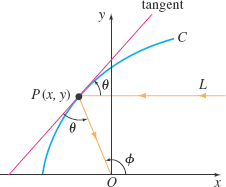
\includegraphics[width=.382\textwidth, right]{lightfocus.png}
\end{figure}

\end{document}